\documentclass[11pt
  , a4paper
  , article
  , oneside
  %  , twoside
  , showtrims
 % , draft
]{memoir}

\usepackage{essdocs}
\usepackage[numbers]{natbib}
\usepackage[autostyle]{csquotes}

%% \usepackage{epstopdf}
%% \usepackage[pdf]{pstricks}
%% \usepackage{graphicx}

\setsecnumdepth{subsection}

\begin{document}
%\frontmatter
%% ESS Document Description
%%
\essdocdesc{Engineering Manual}

%% ESS Document Number
%%
\essdocnum{ESS-XXXXXXXX}

%% Date
%%
\date{\today}

%% ESS Document Revision Number
%%
\essdocrev{0.1}

%% ESS Document State
%%
\essdocstate{Early Draft}

%% ESS Document Classification
%%
\essdocclass{ESS Use Only}

%% Document Title
%%
\title{ICS Engineering Manual}
\subtitle{for MRF MTCA-EVR-300}
%% Document Author(s), if more than one author,
%% use \newline instead of \\ or \linebreak in order to seperate them
\author{Javier Cereijo Garcia \newline Jeong Han Lee }

%% Document Reviewer(s) if more than one reviewer,
%% use \newline instead of \\ or \linebreak in order to seperate them
%\reviewer{Timo Korhonen (Chief Engineer) \newline Timo Korhonen (Chief Engineer)}
\reviewer{TBD}
%% Document Owner(s) if more than one owner,
%% use \newline instead of \\ or \linebreak in order to seperate them
\owner{ICS}

%% Document Approver(s) if more than one approver,
%% use \newline instead of \\ or \linebreak in order to seperate them
\approver{ICS}

\showtrimson

\esstitle
\newpage
\tableofcontents
\newpage

%\mainmatter


%%% Actual Document Start at below
\chapter{Overview}
At European Spallation Source (ESS), Integrated Control System (ICS) does use the Micro Research Finland (MRF) Timing System{\footnote{\url{http://www.mrf.fi/}}} as its timing system of the ESS site. The consistent and up-to-date engineering manual is essential for the ESS Timing system.

\section{Scope}
\begin{itemize}
\item This document identifies one of the MRF Timing Event Receivers (EVR) that needs to be configured for an ESS subsystem that needs synchronous frequencies, trigger signals and sequences of events \cite{MRFEVENTSYSTEMDC}.
\item This document provides the generic description of the MRF MTCA-EVR-300 and its interface board (IFB-300). In addition, it affords the minimal, essential, and generic information for the system configuration.  
\item The purpose of this document is to describe the engineering procedure and troubleshooting about how the MRF MTCA-EVR-300 board will be integrated in cooperation with the ESS EPICS Environment (EEE).
\item This document attempts to maintain consistency with existing ESS Timing system hardware as far as possible. 
\end{itemize}
\textbf{Note that this is a very early draft document and should be updated as development progresses.}

\section{Target Audience}
This document is targeted to ICS engineers and technical stakeholders of the ESS timing system. It is assumed that the target audience has a technical background in the MRF Timing System, the EPICS development, and a Linux environment.

\chapter{System Description}
MRF Technical Reference \citep[see][p45]{MRFEVENTSYSTEMDC} explained Event Receivers and wrote :
\blockquote{\textit{Event Receivers decode timing events and signals from an optical event stream transmitted by an Event Generator. Events and signals are received at predefined rate the event clock that is usually divided down from an accelerators main RF reference. The event receivers lock to the phase event clock of the Event Generator and are thus phase locked to the RF reference. Event Receivers convert event codes transmitted by an Event Generator to hardware outputs. They can also generate software interrupts and store the event codes with globally distributed timestamps into FIFO memory to be read by a CPU.}}

ICS uses and will use the following different types of EVR :
\begin{itemize}
\item VME-EVR-230 / 230RF
\item PMC-EVR-230
\item MTCA-EVR-300 / 300DC
\item PCIe-EVR-300 / 300DC
\item VME-EVR-300 / 300DC
\end{itemize}

The scope of this document is to cover MTCA-EVR-300 board.


\section{MTCA-EVR-300}
Figure~\ref{fig:mtca-evr300} shows the rough physical dimensions $181\times 148~\mathrm{mm}{}^2$ of the MTCA-EVR-300 card.

\begin{figure}[!htb]
  \centering
  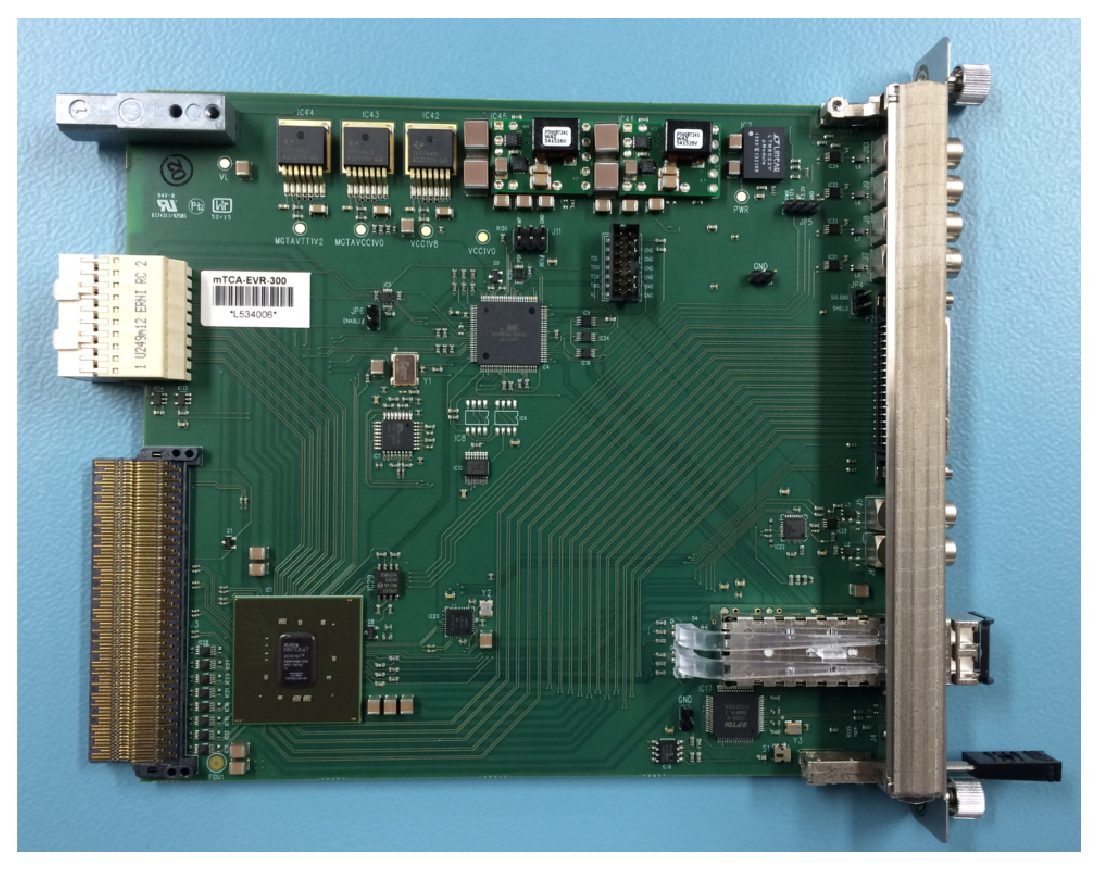
\includegraphics[width=0.99\textwidth]{./pictures/mtca_evr_300.eps}
  \caption{
    MRF MTCA-EVR-300 board.
  }
  \label{fig:mtca-evr300}   
\end{figure}


The MTCA-EVR-300  has a SFP transceiver as an input from EVG and several outputs: 4 front panel outputs, 16 front universal outputs (through the IFB-300 extension board) and 40 rear outputs. The initial 32 rear outputs map to the RTM connector, the last 8 rear outputs map to the MTCA backplane. The 16 front universal outputs are implemented through a micro-SCSI type connector for an interface board IFB-300. The IFB-300 has eight Universal I/O slots, shown in Figure~\ref{fig:ifb-300}. With different type of MRF Universal I/O modules, each slot can be used as an unique trigger or event signal source.

\begin{figure}[!htb]
  \centering
  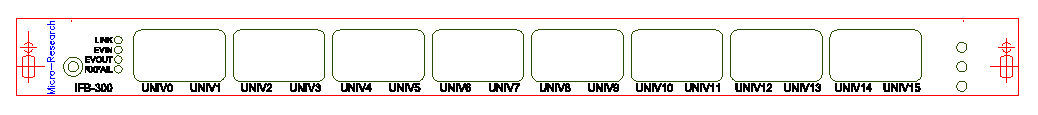
\includegraphics{./pictures/ifb-300.eps}
  \caption{
    MRF Interface Board IFB 300 Front Panel \cite{MRFEVENTSYSTEMDC}.
  }
  \label{fig:ifb-300}   
\end{figure}


\clearpage

\chapter{System Environment}
Before describing the engineering procedure for an EEE integration of the MRF MTCA-EVR-300 board, it is mandatory to have proper system environment that consists of specific hardware and software lists. Here we will show the hardware and software lists, their block diagrams, and their setup in the ICS lab at ESS. The information shown in this chapter is used in the ICS Lab at ESS.


\section{Hardware}
Table~\ref{table:hwlist} shows the hardware list and its environment. The form factor and version of EVG can be changeable. It is assumed that the proper working EVG system is ready. Here, \texttt{TAG} is used as the prefix of the ICS internal inventory system in order to track it down. One can use only EVG without FOUT.
\begin{table}[!hb]
  \centering
  \begin{tabular}{l|l|l}
    \toprule
    Hardware                        & Info                                               & Serial Number \\\midrule
    MRF MTCA-EVR-300                & \texttt{ICS TAG-255}                               & L534006       \\\midrule
    NAT-MCH-PHYS                    & \texttt{ICS TAG-188}                               & 1135150327    \\\midrule
    Concurrent Technologies AMC CPU & \texttt{ICS TAG-190}, hostname: icsb-mtcacpu-ct028 & M2349/028     \\\midrule
    Struck SIS8300                  &                                &      \\\midrule
    ELMA MTCA crate 12 slots, 9U    & \texttt{ICS TAG-181}                               & 10615060      \\\midrule
    Wiener power supply unit 1000W  & \texttt{ICS TAG-187}                               & 0985052       \\\midrule
    MRF IFB-300                     & \texttt{ICS TAG-352}                               & K472044       \\\midrule
    Universal I/O                   &                                                    &               \\\midrule
    MRF cPCI-EVG-230                & \texttt{ICS TAG-26}                                & E283016       \\\midrule
    MRF cPCI-FOUT-12                & \texttt{ICS TAG-27}                                & H385013       \\\midrule
    Optical cables                  & LC, Optical 850 nm                                 &               \\\midrule
    Ethernet cables                 &                                                    &               \\\midrule
    LEMO cables                     &                                                    &               \\\midrule
    LEMO to BNC Adapters            &                                                    &               \\\midrule
    Oscilloscope                    &                                                    &               \\\bottomrule
  \end{tabular}
  \caption[]{Hardware List and Its Environment.}
  \label{table:hwlist}
\end{table}


% Figure~\ref{fig:diagram} shows the physical hardware setup and 
Figure~\ref{fig:mtca-hw-setup} shows the MTCA-EVR-300 setup in the lab. From left to right, the power supply, MCH, CPU, MTCA-EVR-300 and Struck SIS8300.
\begin{figure}[!b]
  \centering
  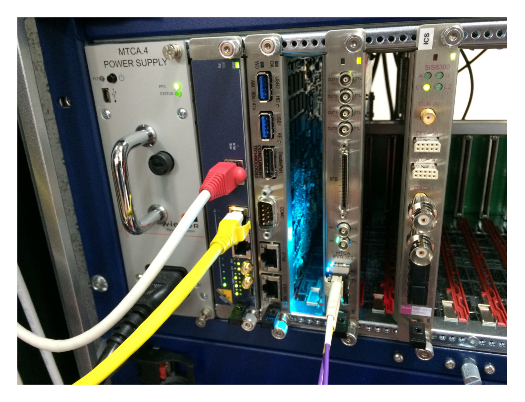
\includegraphics[width=0.8\textwidth]{./pictures/mtca-hw-setup.eps}
  \caption{Hardware Setup in the ICS lab.}
  \label{fig:mtca-hw-setup}   
\end{figure}


\clearpage
\section{Software}
Table~\ref{table:swlist} shows the Software list and its environment. It is mandatory to check the kernel version, and the mrf kernel module version. Since the mrfioc2 is dependent upon devLibs2 EEE internally, an end-user is unnecessary to check its version explicitly. 
\begin{table}[!htb]
  \centering
  \begin{tabular}{l|l}
    \toprule
    Item               & Version Info.                                            \\\midrule
    CentOS Linux       & \texttt{7.1.1503}                                        \\\midrule
    Kernel             & \texttt{3.10.0-229.7.2.el7.x86\_64}                      \\\midrule
    mrf kernel module  & version : \texttt{1} / srcversion \texttt{124F2C1F3D5E2080AE1B755}     \\\midrule
    EEE                & \texttt{1.8.0}                                  \\\midrule
    EPICS Base         & \texttt{3.14.12.5}                              \\\midrule
    mrfioc2            & EEE module ver. \texttt{2.7.13}                 \\\midrule
    devLib2            & EEE module ver. \texttt{2.6+}                   \\\bottomrule
  \end{tabular}
  \caption[]{Software and its version information.}
  \label{table:swlist}
\end{table}

\section{EVR Firmware}
Table~\ref{table:fwinfo} shows EVR FPGA Firmware Version Register.

\begin{table}[!htb]
  \centering
  \begin{tabular}{p{0.3\linewidth}|c|l}
    \toprule
    EVR FPGA Firmware Version Register            & \multicolumn{2}{c}{\texttt{0x18000205}}             \\\midrule
    Board Type      & EVR                         &  \texttt{0x}\underline{\textbf{1}}\texttt{8000205}  \\\midrule
    Form Factor     & mTCA.4                      &  \texttt{0x1}\underline{\textbf{8}}\texttt{000205}  \\\midrule
    EVR Firmware ID & Delay Compensation Firmware &  \texttt{0x1800}\underline{\textbf{02}}\texttt{05}  \\\midrule
    EVR Revision ID & 5                           &  \texttt{0x180002}\underline{\textbf{05}}           \\\bottomrule
  \end{tabular}
  \caption[]{EVR FPGA Firmware Version Register in Reference \citep[see][p66]{MRFEVENTSYSTEMDC}.}
  \label{table:fwinfo}
\end{table}


\clearpage
\chapter{Engineering Procedure}
This chapter provides the minimal information to configure the EVR board properly. 

\section{System Installation}
%Figure~\ref{fig:diagram} and 
Figure~\ref{fig:mtca-hw-setup} shows the glimpse of what system might be like in a Lab. \textbf{Note that the cable between the mTCA-EVR-300DC and IFB-300 (not shown in the figure) should be connected, disconnected, or both only when powered down}. Please see the detail information in Reference \citep[][p54]{MRFEVENTSYSTEMDC}.
  
\section{mTCA-EVR-300 Board Identification}
         
\subsection{Kernel Module}
It is essential to load the mrf kernel module and to check its information as follows:
\begin{lstlisting}[style=termstyle]
[root@icsb-mtcacpu-ct028 mTCA-EVR-300_tests]# modprobe mrf
  
[root@icsb-mtcacpu-ct028 mTCA-EVR-300_tests]# modinfo mrf
filename:       /lib/modules/3.10.0-229.7.2.el7.x86_64/extra/mrf.ko
author:         Michael Davidsaver <mdavidsaver@bnl.gov>
version:        1
license:        GPL v2
rhelversion:    7.1
srcversion:     124F2C1F3D5E2080AE1B755
depends:        parport,uio
vermagic:       3.10.0-229.7.2.el7.x86_64 SMP mod_unload modversions 
parm:           cable:Name of JTAG parallel port cable to emulate (charp)
parm:           interfaceversion:User space interface version (int)
\end{lstlisting}

It is mandatory to check the access permission of an IOC user for the device file, e.g., \path{/dev/uio0} to allow the IOC process to open it. In case ones target system is NOT running \texttt{UDEV}, please consult the EVG user guide~\cite{EVR-USER-GUIDE}. And for building and loading the EVR kernel module and for changing the device file permission, please see Reference~\citep[see][p12,13]{EVR-USER-GUIDE}. It is inadvisable to change the file permission by using \texttt{chmod}. 

\subsection{PCI Addressing}
Each PCI device is identified by a domain, a bus, a device, and a function number in Linux. Therefore, in order to initialize the MRF MTCA-EVR-300 board in EEE, one needs the following information: a domain number, a bus number, a device number, and a function number. These numbers are the parameters of a \texttt{mrmEvrSetupPCI} function.

One can use \texttt{lspci} to find them as follows:
\begin{lstlisting}[style=termstyle]
[root@icsb-mtcacpu-ct028 mTCA-EVR-300_tests]# lspci
...
06:00.0 Signal processing controller: Xilinx Corporation Device 7011
...
[root@icsb-mtcacpu-ct028 mTCA-EVR-300_tests]# lspci -s 06:00 -vv
06:00.0 Signal processing controller: Xilinx Corporation Device 7011
	Subsystem: Device 1a3e:132c
	Physical Slot: 3
	Control: I/O+ Mem+ BusMaster+ SpecCycle- MemWINV- VGASnoop- ParErr- Stepping- SERR- FastB2B- DisINTx-
	Status: Cap+ 66MHz- UDF- FastB2B- ParErr- DEVSEL=fast >TAbort- <TAbort- <MAbort- >SERR- <PERR- INTx-
	Latency: 0, Cache Line Size: 64 bytes
	Interrupt: pin A routed to IRQ 18
	Region 0: Memory at c0700000 (32-bit, non-prefetchable) [size=256K]
	Capabilities: [40] Power Management version 3
		Flags: PMEClk- DSI+ D1- D2- AuxCurrent=0mA PME(D0-,D1-,D2-,D3hot-,D3cold-)
		Status: D0 NoSoftRst+ PME-Enable- DSel=0 DScale=0 PME-
	Capabilities: [48] MSI: Enable- Count=1/1 Maskable- 64bit+
		Address: 0000000000000000  Data: 0000
	Capabilities: [60] Express (v2) Endpoint, MSI 00
		DevCap:	MaxPayload 256 bytes, PhantFunc 1, Latency L0s <64ns, L1 <1us
			ExtTag+ AttnBtn- AttnInd- PwrInd- RBE+ FLReset-
		DevCtl:	Report errors: Correctable- Non-Fatal- Fatal- Unsupported-
			RlxdOrd+ ExtTag- PhantFunc- AuxPwr- NoSnoop+
			MaxPayload 256 bytes, MaxReadReq 512 bytes
		DevSta:	CorrErr- UncorrErr- FatalErr- UnsuppReq- AuxPwr- TransPend-
		LnkCap:	Port #0, Speed 2.5GT/s, Width x1, ASPM L0s, Exit Latency L0s unlimited, L1 unlimited
			ClockPM- Surprise- LLActRep- BwNot-
		LnkCtl:	ASPM Disabled; RCB 64 bytes Disabled- CommClk-
			ExtSynch- ClockPM- AutWidDis- BWInt- AutBWInt-
		LnkSta:	Speed 2.5GT/s, Width x1, TrErr- Train- SlotClk+ DLActive- BWMgmt- ABWMgmt-
		DevCap2: Completion Timeout: Not Supported, TimeoutDis-, LTR-, OBFF Not Supported
		DevCtl2: Completion Timeout: 50us to 50ms, TimeoutDis-, LTR-, OBFF Disabled
		LnkCtl2: Target Link Speed: 2.5GT/s, EnterCompliance- SpeedDis-
			 Transmit Margin: Normal Operating Range, EnterModifiedCompliance- ComplianceSOS-
			 Compliance De-emphasis: -6dB
		LnkSta2: Current De-emphasis Level: -3.5dB, EqualizationComplete-, EqualizationPhase1-
			 EqualizationPhase2-, EqualizationPhase3-, LinkEqualizationRequest-
	Capabilities: [100 v1] Device Serial Number 00-00-00-00-00-00-00-00
	Kernel driver in use: mrf-pci

\end{lstlisting}

And one should identify four number as follows:
\begin{lstlisting}[style=termstyle]
[root@icsb-mtcacpu-ct028 mTCA-EVR-300_tests]# lspci -s 06:00 -t
-+-[0000:06]---00.0
 \-[0000:00]-
\end{lstlisting}
, where \texttt{-+-[0000:06]---00.0} can be translated to \texttt{-+-}[domain:bus]\texttt{---}device.function. Thus in the above case, four numbers are shown in Table~\ref{table:pciidnumber}.\begin{table}[!htb]
  \centering
  \begin{tabular}{l|l}
    \toprule
    domain   & 0x0 \\\midrule
    bus      & 0x6 \\\midrule
    device   & 0x0 \\\midrule
    function & 0x0 \\\bottomrule
  \end{tabular}
  \caption[]{MRF MTCA-EVR-300 Identification Numbers}
  \label{table:pciidnumber}
\end{table}


\clearpage
\section{EPICS IOC Setup under EEE}
In this section, in order to start the EPICS IOC for the MRF MTCA-EVR-300 under EEE, one should consider the following things: 1) the EPICS database file, and 2) the EPICS start-up script. All files are located in a directory, where an user can create, e.g., in the ICS Lab, 
\begin{lstlisting}[style=termstyle, label={list:pwd}, caption={Working Directory in the ICS lab.} ]
/home/javiercereijogarcia/mTCA-EVR-300_tests
\end{lstlisting}

\subsection{EPICS Database File}
One could use the existent database file in the EEE as a template for the EPICS IOC, the file is located in the following location : 
\begin{lstlisting}[style=termstyle]
/opt/epics/modules/mrfioc2/2.7.13/db/evr-mtca-300.db
\end{lstlisting} 


\subsection{Start-Up Script}
Listing~\ref{list:mTCA-EVR-300_1.cmd} shows the IOC start-up script which has the MRF MTCA-EVR-300 Identification Numbers, shown in Table~\ref{table:pciidnumber}. Note that the start-up script is located in the directory in Listing~\ref{list:pwd}.


\begin{lstlisting}[
    style=termstylenumber,
    label={list:mTCA-EVR-300_1.cmd},
    caption={Start-up script \texttt{mTCA-EVR-300\_1.cmd}. Line \ref{pciid0}-\ref{pciid3} should be matched to Table~\ref{table:pciidnumber}. }
  ]
epicsEnvSet("SYS"             "tests-mTCA-EVR-300")
epicsEnvSet("DEVICE"          "EVR0")
epicsEnvSet("EVR_PCIDOMAIN"   "0x0") (*@\label{pciid0}@*)
epicsEnvSet("EVR_PCIBUS"      "0x6") (*@\label{pciid1}@*)
epicsEnvSet("EVR_PCIDEVICE"   "0x0") (*@\label{pciid2}@*)
epicsEnvSet("EVR_PCIFUNCTION" "0x0") (*@\label{pciid3}@*)

require mrfioc2,2.7.13

mrmEvrSetupPCI($(DEVICE), $(EVR_PCIDOMAIN), $(EVR_PCIBUS), $(EVR_PCIDEVICE), $(EVR_PCIFUNCTION))

dbLoadRecords("evr-mtca-300.db", "DEVICE=$(DEVICE), SYS=$(SYS), Link-Clk-SP=88.0525") (*@\label{dbpwd}@*)
  
\end{lstlisting}

\subsection{EPICS IOC}
Under EEE, the EPICS IOC can be started via the command \texttt{iocsh mTCA-EVR-300\_1.cmd}. The output should look like as follows:

\begin{lstlisting}[style=termstyle]
[root@icsb-mtcacpu-ct028 mTCA-EVR-300_tests]# iocsh mTCA-EVR-300_1.cmd 
/opt/epics/bases/base-3.14.12.5/bin/centos7-x86_64/softIoc -D /opt/epics/bases/base-3.14.12.5/dbd/softIoc.dbd /tmp/iocsh.startup.23209
#date="Fri  9 Sep 13:52:57 UTC 2016"
#user="javiercereijogarcia"
#PWD="/home/javiercereijogarcia/mTCA-EVR-300_tests"
#EPICSVERSION="3.14.12.5"
#EPICS_HOST_ARCH="centos7-x86_64"
#SHELLBOX=""
#EPICS_CA_ADDR_LIST=""
#EPICS_MODULE_INCLUDE_PATH=".:/usr/lib64:/usr/lib:/lib64:/lib"
dlload         /opt/epics/modules/environment/1.8.0/3.14.12.5/lib/centos7-x86_64/libenvironment.so
dbLoadDatabase /opt/epics/modules/environment/1.8.0/3.14.12.5/dbd/environment.dbd
environment_registerRecordDeviceDriver
< "mTCA-EVR-300_1.cmd"
epicsEnvSet("SYS"             "tests-mTCA-EVR-300")
epicsEnvSet("DEVICE"          "EVR0")
epicsEnvSet("EVR_PCIDOMAIN"   "0x0")
epicsEnvSet("EVR_PCIBUS"      "0x6")
epicsEnvSet("EVR_PCIDEVICE"   "0x0")
epicsEnvSet("EVR_PCIFUNCTION" "0x0")
require mrfioc2,2.7.13
require: mrfioc2 depends on devlib2 (2.6+).
require: Loading library /opt/epics/modules/devlib2/2.6.0/3.14.12.5/lib/centos7-x86_64/libdevlib2.so.
require: Loading /opt/epics/modules/devlib2/2.6.0/3.14.12.5/dbd/devlib2.dbd.
require: Calling devlib2_registerRecordDeviceDriver function.
require: Loading library /opt/epics/modules/mrfioc2/2.7.13/3.14.12.5/lib/centos7-x86_64/libmrfioc2.so.
require: Adding /opt/epics/modules/mrfioc2/2.7.13/db.
require: Adding /opt/epics/modules/mrfioc2/2.7.13/startup.
require: Loading /opt/epics/modules/mrfioc2/2.7.13/3.14.12.5/dbd/mrfioc2.dbd.
require: Calling mrfioc2_registerRecordDeviceDriver function.
 
mrmEvrSetupPCI(EVR0, 0x0, 0x6, 0x0, 0x0)
Device EVR0 6:0.0
Using IRQ 18
Setting magic LE number!
FPGA version 0x18000205
Firmware version: 00000205
Found EVR0:SFP0 SFP transceiver
Flash access: this form factor is not supported.
MTCA: Out FP:4 FPUNIV:16 RB:40 IFP:2 GPIO:0
dbLoadRecords("evr-mtca-300.db", "DEVICE=EVR0, SYS=tests-mTCA-EVR-300, Link-Clk-SP=88.0525")
iocInit
Starting iocInit
############################################################################
## EPICS R3.14.12.5-2015-08 $Date: Tue 2015-03-24 09:57:35 -0500$
## EPICS Base built Oct  9 2015
############################################################################
Set EVR clock 88052500.000000
iocRun: All initialization complete
epicsEnvSet IOCSH_PS1,"icsb-mtcacpu-ct028> "
icsb-mtcacpu-ct028>
\end{lstlisting}

In addition, the PCI information is available within the running IOC via \texttt{devPCIShow} as follows:
\begin{lstlisting}
icsb-mtcacpu-ct028> devPCIShow
Look for the line with your configuration information, in our case is:
PCI 0000:06:00.0 IRQ 18
  vendor:device 10ee:7011 rev 00
Where the vendor id 10ee is Xilinx Corporation.
And show the PCI information with (the second parameter is the verbosity level):
icsb-mtcacpu-ct028> devPCIShow 9 0x10ee
PCI 0000:06:00.0 IRQ 18
  vendor:device 10ee:7011 rev 00
  subved:subdev 1a3e:132c
  class 118000 generic signal processing controller
  driver mrf-pci
  BAR 0 32-bit MMIO    256 kB
Matched 1 devices
icsb-mtcacpu-ct028>
\end{lstlisting}

\newpage
\chapter{System In-Situ Verification Procedure}
This chapter provides the minimal system verification procedure. If one wants to do more step-by-step procedure which may be useful when testing the function of hardware and software, please see Reference~~\citep[see][p14]{EVR-USER-GUIDE}.

\begin{table}[!htb]
  \centering
  \begin{tabular}{c|p{0.4\linewidth}|p{0.42\linewidth}}
    \toprule
    Step & Goal                                       & Info.                                                  \\\midrule
    1    & Check the EVR \& EVR connection            & Link status, link clock, and heartbeat timeout counter \\\midrule
    2    & Monitor Receiving and acknowledging Events & Event counter and receiving event frequency            \\\midrule
    3    & Generate Trigger Signals from EVR          & Various trigger signals with an oscilloscope           \\\bottomrule
  \end{tabular}
  \caption[]{System In-Situ Verification Procedure}
  \label{table:checklist}
\end{table}


\section{Step 1 : Check the EVR and EVR connection}
Short comments on each command or a series of commands are shown before the corresponding command.
\begin{lstlisting}[style=termstyle]
#
# We can check the EVG and EVR link status and the link clock setting, and can also see the link down counter as well.
#
[user@host ~]$ caget tests-mTCA-EVR-300-EVR0:Link-Sts
tests-mTCA-EVR-300-EVR0:Link-Sts OK
[user@host ~]$ caget tests-mTCA-EVR-300-EVR0:Link-Clk-I
tests-mTCA-EVR-300-EVR0:Link-Clk-I 88.0519
#
# Change the wrong clock setting on EVR, then we expect that the link status will be Fail.  
#
[user@host ~]$ caput tests-mTCA-EVR-300-EVR0:Link-Clk-SP 100
Old : tests-mTCA-EVR-300-EVR0:Link-Clk-SP 88.0525
New : tests-mTCA-EVR-300-EVR0:Link-Clk-SP 100
[user@host ~]$ caget tests-mTCA-EVR-300-EVR0:Link-Sts
tests-mTCA-EVR-300-EVR0:Link-Sts Fail
[user@host ~]$ caget tests-mTCA-EVR-300-EVR0:Link-Clk-I
tests-mTCA-EVR-300-EVR0:Link-Clk-I 100
#
# Revert it back to the proper clock setting, and the link status will be OK.
#
[user@host ~]$ caput tests-mTCA-EVR-300-EVR0:Link-Clk-SP 88.0525
Old : tests-mTCA-EVR-300-EVR0:Link-Clk-SP 100
New : tests-mTCA-EVR-300-EVR0:Link-Clk-SP 88.0525
[user@host ~]$ caget tests-mTCA-EVR-300-EVR0:Link-Sts
tests-mTCA-EVR-300-EVR0:Link-Sts OK
#
# There is a link heartbeat counter that gets updated aproximately every 1.3 s when the link is off. Camonitor it to check its functionality.
#
[user@host ~]$ camonitor tests-mTCA-EVR-300-EVR0:Cnt-LinkTimo-I
tests-mTCA-EVR-300-EVR0:Cnt-LinkTimo-I 2016-09-12 11:49:11.463914 35
#
# Open another terminal, to change the wrong link clock. 
#
[user@host ~]$ caput tests-mTCA-EVR-300-EVR0:Link-Clk-SP 100
Old : tests-mTCA-EVR-300-EVR0:Link-Clk-SP 88.0525
New : tests-mTCA-EVR-300-EVR0:Link-Clk-SP 100
#
# The heartbeat counter should be increasing as follows: 
#
tests-mTCA-EVR-300-EVR0:Cnt-LinkTimo-I 2016-09-12 11:50:06.760264 36  
tests-mTCA-EVR-300-EVR0:Cnt-LinkTimo-I 2016-09-12 11:50:08.056687 37  
tests-mTCA-EVR-300-EVR0:Cnt-LinkTimo-I 2016-09-12 11:50:09.353116 38  
tests-mTCA-EVR-300-EVR0:Cnt-LinkTimo-I 2016-09-12 11:50:10.649505 39  
tests-mTCA-EVR-300-EVR0:Cnt-LinkTimo-I 2016-09-12 11:50:11.945937 40 
#
# The counter will be stopped after the proper value is given.
# 
\end{lstlisting}

\section{Step 2 : Monitor Receiving and acknowledging Events}
For this step, an additional EVR database file is needed to add to the end line of the \path{mTCA-EVR-300_1.cmd} file. The new start-up script file, \path{mTCA-EVR-300_2.cmd} is shown in Listing~\ref{list:mTCA-EVR-300_2.cmd}. 
\begin{lstlisting}[
    style=termstylenumber,
    label={list:mTCA-EVR-300_2.cmd},
    caption={Start-up script \texttt{mTCA-EVR-300\_2.cmd}. }
  ]
epicsEnvSet("SYS"             "tests-mTCA-EVR-300")
epicsEnvSet("DEVICE"          "EVR0")
epicsEnvSet("EVR_PCIDOMAIN"   "0x0")
epicsEnvSet("EVR_PCIBUS"      "0x6")
epicsEnvSet("EVR_PCIDEVICE"   "0x0")
epicsEnvSet("EVR_PCIFUNCTION" "0x0")

require mrfioc2,2.7.13

mrmEvrSetupPCI($(DEVICE), $(EVR_PCIDOMAIN), $(EVR_PCIBUS), $(EVR_PCIDEVICE), $(EVR_PCIFUNCTION))

dbLoadRecords("evr-mtca-300.db", "DEVICE=$(DEVICE), SYS=$(SYS), Link-Clk-SP=88.0525")

dbLoadRecords("evr-softEvent.template", "DEVICE=$(DEVICE), SYS=$(SYS), EVT=14, CODE=14")
\end{lstlisting}

Short comments on each command or a series of commands are shown before the corresponding command.

\begin{lstlisting}[style=termstylenumber]
#
# start the IOC
#
user@host:~$ iocsh mTCA-EVR-300_2.cmd

#
# Monitor the Event counter with 14 and check the time difference between counters, e.g., 278 and 279, is 0.071429s, i.e., 14 Hz.
# In another terminal:
[user@host ~]$ camonitor tests-mTCA-EVR-300-EVR0:Event-14-Cnt-I
tests-mTCA-EVR-300-EVR0:Event-14-Cnt-I 2016-09-12 11:52:57.724374 278  
tests-mTCA-EVR-300-EVR0:Event-14-Cnt-I 2016-09-12 11:52:57.795803 279  
tests-mTCA-EVR-300-EVR0:Event-14-Cnt-I 2016-09-12 11:52:57.867231 280  
tests-mTCA-EVR-300-EVR0:Event-14-Cnt-I 2016-09-12 11:52:57.938660 281  
tests-mTCA-EVR-300-EVR0:Event-14-Cnt-I 2016-09-12 11:52:58.010099 282
\end{lstlisting}


\section{Step 3 : Generate Trigger Signals from EVR}
In this step output triggers will be generated after receiving an event from the event generator. The mTCA-EVR-300 has 3 types of outputs: 4 front panel outputs, 16 front universal outputs (through the IFB-300 extension board) and 40 rear outputs. The front and front universal outputs can be checked with an oscilloscope, and the rear outputs with an AMC capable of acknowledging the triggers, such as a data acquisition board Struck SIS8300.

The start-up script file for the front and front universal outputs, \path{mTCA-EVR-300_3.cmd} is shown in Listing~\ref{list:mTCA-EVR-300_3.cmd}. 
\begin{lstlisting}[ 
    style=termstylenumber,
    label={list:mTCA-EVR-300_3.cmd},
    caption={Start-up script \texttt{mTCA-EVR-300\_3.cmd}.}
  ]
epicsEnvSet("SYS"             "tests-mTCA-EVR-300")
epicsEnvSet("DEVICE"          "EVR0")
epicsEnvSet("EVR_PCIDOMAIN"   "0x0")
epicsEnvSet("EVR_PCIBUS"      "0x6")
epicsEnvSet("EVR_PCIDEVICE"   "0x0")
epicsEnvSet("EVR_PCIFUNCTION" "0x0")

require mrfioc2,2.7.13

mrmEvrSetupPCI($(DEVICE), $(EVR_PCIDOMAIN), $(EVR_PCIBUS), $(EVR_PCIDEVICE), $(EVR_PCIFUNCTION))

dbLoadRecords("evr-mtca-300.db", "DEVICE=$(DEVICE), SYS=$(SYS), Link-Clk-SP=88.0525")

dbLoadRecords("evr-softEvent.template", "DEVICE=$(DEVICE), SYS=$(SYS), EVT=14, CODE=14")

dbLoadRecords("evr-pulserMap.template", "DEVICE=$(DEVICE), SYS=$(SYS), PID=0, F=Trig, ID=0, EVT=14")  
dbLoadRecords("evr-pulserMap.template", "DEVICE=$(DEVICE), SYS=$(SYS), PID=1, F=Trig, ID=0, EVT=14")  
\end{lstlisting}

An EVR is composed of several logical sub-units, and one of the logical sub-units is the pulse generator. Each pulse generator has an associated Delay and Width \cite{EVR-USER-GUIDE}. In the following procedure, two pulse generators are mapped to the \path{OUT0} and \path{OUT2} of IFB-300, which are connected to the channel 1 and 2 of the oscilloscope respectively in order to see whether output signals are generated according to Delay's and Width's changes. Short comments on each command or a series of commands are shown before the corresponding command.

\subsection{\texttt{OUT0} output}
\begin{lstlisting}[style=termstyle]
#
# Start the IOC
#
user@host:~$ iocsh mTCA-EVR-300_3.cmd

#
# Open a new terminal and set the Pulse generator 0 to the OUT0 output
# 
user@host:~$ caput tests-mTCA-EVR-300-EVR0:FrontOut0-Src-SP 0
Old : tests-mTCA-EVR-300-EVR0:FrontOut0-Src-SP 63
New : tests-mTCA-EVR-300-EVR0:FrontOut0-Src-SP 0

#
# Set the trigger event 14 to the pulse generator 0
#
user@host:~$ caput tests-mTCA-EVR-300-EVR0:Pul0-Evt-Trig0-SP 14
Old : tests-mTCA-EVR-300-EVR0:Pul0-Evt-Trig0-SP    14
New : tests-mTCA-EVR-300-EVR0:Pul0-Evt-Trig0-SP    14

#
# Set the width time of the pulse generator 0. 10 000 is translated to 10 ms.
#
user@host:~$ caput tests-mTCA-EVR-300-EVR0:Pul0-Width-SP 10000
Old : tests-mTCA-EVR-300-EVR0:Pul0-Width-SP        0
New : tests-mTCA-EVR-300-EVR0:Pul0-Width-SP        10000
\end{lstlisting}
Figure~\ref{fig:14Hz} shows the output of \texttt{OUT0} in an oscilloscope. 
\begin{figure}[!ht]
  \centering
    \includegraphics[width=0.8\textwidth]{./pictures/img_1965.eps}
  \caption{14 Hz signal with 10 ms width}
  \label{fig:14Hz}
\end{figure}


\subsection{Width Time of Pulse Generator}

\begin{lstlisting}[style=termstyle]
#
# Change the width time of the pulse generator 0 from 10 ms to 50 ms
#
user@host:~$ caput tests-mTCA-EVR-300-EVR0:Pul0-Width-SP 50000
Old : tests-mTCA-EVR-300-EVR0:Pul0-Width-SP        10000
New : tests-mTCA-EVR-300-EVR0:Pul0-Width-SP        50000  
\end{lstlisting}
and the output is shown in Figure~\ref{fig:50ms}.
\begin{figure}[!ht]
  \centering
    \includegraphics[width=0.78\textwidth]{./pictures/img_1966.eps}
  \caption{14 Hz signal with 50 ms width}
  \label{fig:50ms}
\end{figure}

\subsection{Delay Time of Pulse Generator}
\begin{lstlisting}[style=termstyle]
#
# Set the width time - 20 ms - of the pulse generator 0 
#
user@host:~$ caput tests-mTCA-EVR-300-EVR0:Pul0-Width-SP 20000
Old : tests-mTCA-EVR-300-EVR0:Pul0-Width-SP        50000
New : tests-mTCA-EVR-300-EVR0:Pul0-Width-SP        20000

#
# Set the Pulse generator 1 to the OUT2 output
# 
user@host:~$ caput tests-mTCA-EVR-300-EVR0:FrontOut2-Src-SP 1
Old : tests-mTCA-EVR-300-EVR0:FrontOut2-Src-SP 63
New : tests-mTCA-EVR-300-EVR0:FrontOut2-Src-SP 0

#
# Set the trigger event 14 to the pulse generator 1
#
user@host:~ $ caput tests-mTCA-EVR-300-EVR0:Pul1-Evt-Trig0-SP 14
Old : tests-mTCA-EVR-300-EVR0:Pul1-Evt-Trig0-SP    14
New : tests-mTCA-EVR-300-EVR0:Pul1-Evt-Trig0-SP    14

#
# Set the width time - 20 ms - of the pulse generator 1 
#
user@host:~$ caput tests-mTCA-EVR-300-EVR0:Pul1-Width-SP 20000
Old : tests-mTCA-EVR-300-EVR0:Pul1-Width-SP        0
New : tests-mTCA-EVR-300-EVR0:Pul1-Width-SP        20000

#
# Set the delay time - 30 ms - of the pulse generator 1 
#
user@host:~$ caput tests-mTCA-EVR-300-EVR0:Pul1-Delay-SP 30000
Old : tests-mTCA-EVR-300-EVR0:Pul1-Delay-SP        0
New : tests-mTCA-EVR-300-EVR0:Pul1-Delay-SP        30000
\end{lstlisting}
Figure~\ref{fig:delay} shows the result.
\begin{figure}[!htb]
  \centering
    \includegraphics[width=0.78\textwidth]{./pictures/img_1982.eps}
  \caption{Two 14 Hz signals with 30 ms delay}
  \label{fig:delay}
\end{figure}


\subsection{\texttt{UNIV2} output}
The \path{UNIV0} to \path{UNIV15} outputs in the IFB-300 board work just in the same way as \path{OUT0} to \path{OUT3}. To set the pulse generator 0 to the \path{UNIV2} output do:
\begin{lstlisting}[style=termstyle]
#
# Set the Pulse generator 0 to the UNIV2 output
# 
user@host:~$ caput tests-mTCA-EVR-300-EVR0:FrontUnivOut2-Src-SP 0
Old : tests-mTCA-EVR-300-EVR0:FrontUnivOut2-Src-SP 63
New : tests-mTCA-EVR-300-EVR0:FrontUnivOut2-Src-SP 0
\end{lstlisting}
And set the pulser 0 parameters in the same way as in the previous section. The outputs shown in the oscilloscope should be the same.

\subsection{Rear outputs}
The mTCA-EVR-300 has 40 rear outputs. The initial 32 rear outputs map to the RTM connector, the last 8 rear outputs map to the mTCA backplane. Next it will be shown how to use the rear outputs to trigger the data acquisition in in a Struck SIS8300 board.

The start-up script file for this is \path{mTCA-EVR-300_4.cmd}, shown in Listing~\ref{list:mTCA-EVR-300_4.cmd}. 
\begin{lstlisting}[ 
    style=termstylenumber,
    label={list:mTCA-EVR-300_4.cmd},
    caption={Start-up script \texttt{mTCA-EVR-300\_4.cmd}.}
  ]
epicsEnvSet("SYS"             "EVRTEST")
epicsEnvSet("DEVICE"          "EVRMTCA")
epicsEnvSet("EVR_PCIDOMAIN"   "0x0")
epicsEnvSet("EVR_PCIBUS"      "0x6")
epicsEnvSet("EVR_PCIDEVICE"   "0x0")
epicsEnvSet("EVR_PCIFUNCTION" "0x0")

require recsync
dbLoadRecords(reccaster.db, "P=EVRTEST:recsync:")

require mrfioc2

mrmEvrSetupPCI($(DEVICE), $(EVR_PCIDOMAIN), $(EVR_PCIBUS), $(EVR_PCIDEVICE), $(EVR_PCIFUNCTION))

dbLoadRecords("evr-mtca-300.db", "DEVICE=$(DEVICE), SYS=$(SYS), Link-Clk-SP=88.0525")

dbLoadRecords("evr-softEvent.template", "DEVICE=$(DEVICE), SYS=$(SYS), EVT=14, CODE=14")

dbLoadRecords("evr-pulserMap.template", "DEVICE=$(DEVICE), SYS=$(SYS), PID=0, F=Trig, ID=0, EVT=14")

require sis8300

epicsEnvSet("BUFSIZE", "1024")

ndsCreateDevice("sis8300", "SIS8300", "FILE=/dev/sis8300-5")

dbLoadRecords("sis8300.db", "PREFIX=EVRTEST:DAQ, ASYN_PORT=SIS8300, AI_NELM=1024")
\end{lstlisting}

The line 
\begin{lstlisting}[style=termstyle]
ndsCreateDevice("sis8300", "SIS8300", "FILE=/dev/sis8300-5")
\end{lstlisting}
should be changed according the slot occupied by the SIS8300 board, in this case slot 5 of the mTCA crate. It can be checked by:
\begin{lstlisting}[style=termstyle]
[root@icsb-mtcacpu-ct028 mTCA-EVR-300_tests]# ls /dev/sis8300-*
\end{lstlisting}

To check that the SIS8300 board gets the trigger from the backplane we will run a CSS BOY screen located in
\begin{lstlisting}[style=termstyle]
/opt/epics/modules/sis8300/1.12.1/opi/sis8300.opi
\end{lstlisting}
which is showed in Figure~\ref{fig:OPI}.
\begin{figure}[!htb]
  \centering
    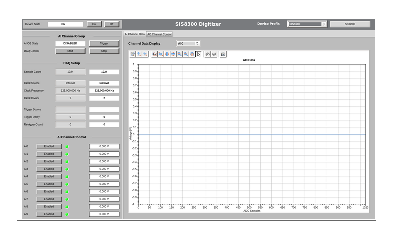
\includegraphics[width=0.78\textwidth]{./pictures/sis8300-digitizer-opi.eps}
  \caption{SIS8300 data acquisition OPI screen.}
  \label{fig:OPI}
\end{figure}

For CSS to work the machine running it should be in the same network as the mTCA crate and have the EEE filesystem. The ESS Development Machine meets these requirements if the PC running it is in the EEE network and connected via VPN to the ICS lab; it's also necessary to set the \texttt{EPICS\_CA\_ADDR\_LIST} field in the CSS preferences to the IP address of the mTCA CPU.

CSS can be launched with the necessary parameters by:
\begin{lstlisting}[style=termstyle]
css --launcher.openFile "/opt/epics/modules/sis8300/1.12.1/opi/sis8300.opi Device2Macro=EVRTEST[\58]DAQ"
\end{lstlisting}

In AI Channel Control, enable AI0, and set Trigger Source \texttt{backplane 1} in the DAQ Setup. Click the button DAQ Control \texttt{Start} under AI Channel Group to put the SIS8300 in a waiting for trigger state. Note that the graph is empty.

Start the IOC and:
\begin{lstlisting}[style=termstyle]
#
# Disable Rear Universal Output 33
# 
[javiercereijogarcia@javcerwin ~]$ caput EVRTEST-EVRMTCA:RearUniv33-Ena-SP "Disabled"
Old : EVRTEST-EVRMTCA:RearUniv33-Ena-SP Enabled
New : EVRTEST-EVRMTCA:RearUniv33-Ena-SP Disabled
#
# Map Rear Universal Output 33 to pulser o
#
[javiercereijogarcia@javcerwin ~]$ caput EVRTEST-MTCAEVR:RearUniv33-Src-SP 0
Old : EVRTEST-MTCAEVR:RearUniv33-Src-SP 63
New : EVRTEST-MTCAEVR:RearUniv33-Src-SP 0
#
# Map pulser 0 to event 14
#
[javiercereijogarcia@javcerwin ~]$ caput EVRTEST-EVRMTCA:Pul0-Evt-Trig0-SP 14
Old : EVRTEST-EVRMTCA:Pul0-Evt-Trig0-SP    14
New : EVRTEST-EVRMTCA:Pul0-Evt-Trig0-SP    14
#
# Set pulser 0 width to 10 ms
#
[javiercereijogarcia@javcerwin ~]$ caput EVRTEST-EVRMTCA:Pul0-Width-SP 10000
Old : EVRTEST-EVRMTCA:Pul0-Width-SP        0
New : EVRTEST-EVRMTCA:Pul0-Width-SP        10000
#
# Watch closely to the graph in the CSS OPI screen when enabling Rear Universal Output 33, since in the next event 14 received the SIS8300 will start the data acquisition; since it is not connected, the data acquired is just 0
#
[javiercereijogarcia@javcerwin ~]$ caput EVRTEST-EVRMTCA:RearUniv33-Ena-SP "Enabled"
Old : EVRTEST-EVRMTCA:RearUniv33-Ena-SP Disabled
New : EVRTEST-EVRMTCA:RearUniv33-Ena-SP Enabled
\end{lstlisting}
RearUniv33 is used to trigger \texttt{backplane 1} because there is an offset of 32 rear outputs in the mTCA-EVR-300 which are mapped to the RTM connector.

\clearpage

\backmatter
%\bibliographystyle{unsrt}
%\bibliographystyle{plainnat}
%\bibliographystyle{abbrvnat}
\bibliographystyle{unsrtnat}
%\bibliographystyle{chicago}
%\bibliography{./ess_refs}
\bibliography{em_mtcaevr300}

\end{document}

